
\label{chap:results}

The main results of this thesis are grouped into three different sections according to the studied phenomena and the used methods. Sections \ref{sec:results_anharm} and \ref{sec:results_interference} summarize the results of non-equilibrium molecular dynamics (NEMD) modeling of lattice heat transfer in various geometries, focusing on anharmonic scattering and wave interference phenomena, respectively. Section \ref{sec:results_gf} highlights the Green's function (GF) approach to modeling quantum effects in phonon transport and the cavity-enhancement of electromagnetic energy transfer.

\section{Anharmonic effects in phononic thermal conduction}
\label{sec:results_anharm}

Phonon-phonon scattering arises from the anharmonic terms in the interatomic potential as discussed in Sec. \ref{sec:th_eom2}. These terms are crucial in first-principles modeling of thermal conduction at interfaces and bulk, because they boost heat transfer across interfaces \cite{lyeo06} and are responsible for the thermal resistivity of pristine bulk materials. Combining NEMD and the spectral decomposition formula \eqref{eq:th_spectral_curr} for the heat current, one can extract detailed information of the effects of these non-linear terms on thermal conduction. Subsection \ref{sec:results_interface} studies the heat current spectrum at the interface between two mass-mismatched materials at different temperatures, revealing two different heat transfer mechanisms relying on anharmonic effects. Subsection \ref{sec:results_mfps} investigates the dependence of the spectral heat current on the tube length in carbon nanotubes, allowing for determining phonon mean free paths at each vibrational frequency. 

Finally, NEMD is used in Subsection \ref{sec:results_twinning} to investigate the effects of periodic twinning on the thermal conductivity in silicon nanowires. Twinning stacking faults are common defects occurring in the vapor-liquid-solid growth of semiconductor nanowires \cite{johansson06,xiong06,davidson07,algra08}, and while their applicability in the tuning of electronic \cite{ikonic93b} and optical \cite{ikonic95} properties has already been demonstrated \cite{im14}, their effect on the thermal properties of nanowires is unknown. The results described in Subsection \ref{sec:results_twinning} suggest that periodic twinning can increase the thermoelectric figure of merit of silicon nanowires. 

\subsection{Interfacial thermal conduction}
\label{sec:results_interface}

The role of anharmonic phonon scattering in interfacial thermal conduction was investigated in \citepub{spectral} using the computational setup presented earlier in Fig. \ref{fig:th_spectral_geom}. Atoms with masses $m_{\textrm{Ar}}=28$ amu (atomic mass of argon) and $4m_{\textrm{Ar}}$ were placed to fill two half-spaces in a face-centered cubic lattice, with the atoms of the two half-spaces being separated by a plane with surface normal along the [100] direction as depicted in Fig. \ref{fig:th_spectral_geom}. The mass-mismatch induces an acoustic mismatch between the materials, creating a non-zero contact resistance for phonons. Interatomic interactions were modeled using the Lennard-Jones potential \cite{allentildesley} and the interaction parameters were chosen to correspond to solid argon \cite{allentildesley}. \change{The bath temperature difference $\Delta T=T_L-T_R$ was set to $\Delta T=T/3$ in all simulations. We carefully checked that the conductance spectra did not visibly change when $\Delta T$ was reduced, ensuring that non-linear contributions to the heat current [proportional to $(\Delta T)^2$ and higher powers of $\Delta T$] were negligible.}

\begin{figure}[tb]
 \begin{center}
  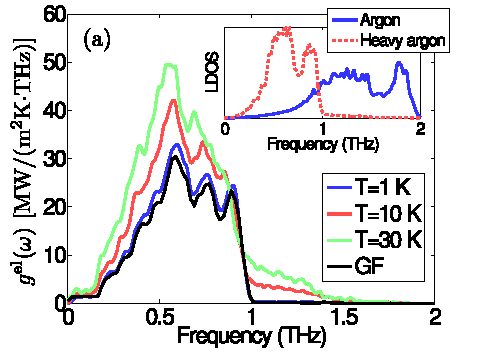
\includegraphics[width=.49\columnwidth]{pics/nemd_fig4a.pdf}
  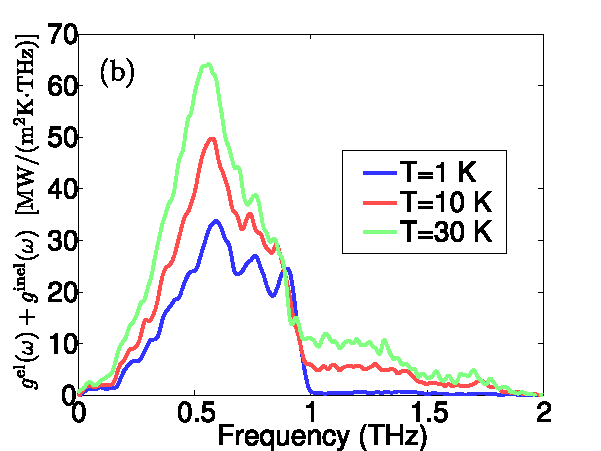
\includegraphics[width=.49\columnwidth]{pics/nemd_fig4b.pdf}
  \caption{Elastic thermal conductance $g^{\textrm{el}}(\omega)=q(\omega)/\Delta T_b$ through the acoustically mismatched interface as a function of frequency at various temperatures.  At $T=1$ K, the elastic conductance agrees with the Landauer-B\"uttiker conductance calculated using the GF method. At high temperatures, anharmonic scattering in the bulk enables energy transfer even above the cut-off frequency of the heavier solid, located at 1 THz.  Inset: Local density of vibrational states (LDOS, arbitrary units) at the interface. (b) The sum $g^{\textrm{el}}(\omega)+ g^{\textrm{inel}}(\omega)$ of elastic and inelastic spectral conductance as a function of frequency. The inelastic conductance describes energy transfer by phonon-phonon interactions across the interface and is defined in detail in \citepub{spectral}. At high temperatures, the anharmonic energy transfer processes strongly enhance interfacial heat transfer at $f\approx 0.5$ THz and above the cut-off of the heavier material (1 THz). Figure reprinted with publisher's permission from \citepub{spectral}.} 
 \label{fig:nemd_fig2}
 \end{center}
\end{figure}

Figure \ref{fig:nemd_fig2}(a) shows the elastic spectral conductance $g^{\textrm{el}}(\omega)=q(\omega)/\Delta T_b$, defined as the first-order contribution to the spectral current $q(\omega)$ [Eq. \eqref{eq:th_spectral_curr}] calculated at the interface divided by the temperature jump $\Delta T_b$. Conductance $g^{\textrm{el}}(\omega)$ is referred to as elastic, because it is calculated from the coupling of vibrations at the same frequency $\omega$ at different sides of the interface. The first-order conductance accounts, however, also for inelastic effects through the non-linear phonon dynamics calculated from NEMD with all orders of interactions. 

As seen in Fig. \ref{fig:nemd_fig2}(a), modes with frequencies above 1 THz cannot carry energy across the interface at low temperature ($T=1$ K), because there are no propagating modes in the heavier material above 1 THz. This absence of modes is evident in the interfacial density of states depicted in the inset of Fig. \ref{fig:nemd_fig2}(a), where only a small tail induced by the evanescent modes is visible above 1 THz in the heavy material. At higher temperatures ($T=10$ K and $T=30$ K), the onset of anharmonic effects can be seen to enable evanescent energy transfer across the interface. Most notably, anharmonic effects enable energy transfer even above the cut-off frequency of the heavier material. These high-frequency modes are evanescent in the heavier material, but they can dissipate their heat to lower-frequency modes in the immediate vicinity of the interface through anharmonic interactions. Our results are the first to explicitly demonstrate energy transfer across interfaces by such evanescent wave dissipation.

To further probe the role of anharmonic scattering in interfacial energy transfer, we determined also the first-order anharmonic contribution to the spectral heat current at the interface. The expression for this first-order anharmonic conductance $g^{\textrm{inel}}(\omega)$, which is referred to as inelastic due to its natural interpretation as describing three-phonon energy transfer processes, was derived from the second-order contribution to spectral heat current as detailed in \citepub{spectral}. The sum of elastic and inelastic contributions to the conductance is shown in Fig. \ref{fig:nemd_fig2}(b). Comparison to Fig. \ref{fig:nemd_fig2}(a) shows that the three-phonon energy transfer processes enhance energy transfer across the whole frequency range between zero and 2 THz, both below and above the cut-off frequency of the heavy argon. As discussed in detail in \citepub{spectral}, these inelastic energy transfer processes are dominated by frequency-doubling and frequency-halving anharmonic processes at the interface, thereby supporting the phenomenological higher harmonic inelastic model suggested earlier by Hopkins \cite{hopkins09_jap}. Because of the high computational burden required for determining the contributions of higher-order anharmonic processes to the conductance and the complexity of analyzing such terms, the analysis of \citepub{spectral} was limited to first-order anharmonic processes.

Our results are the first to quantify the contributions of anharmonic processes to interfacial energy transfer from atomistic simulations and have facilitated the physical interpretation of experimental results for the interfacial conductance between metals and diamond \cite{hohensee15}. 

\subsection{Mean free paths in carbon nanotubes}

\label{sec:results_mfps}

\begin{figure}[tb]
 \begin{center}
  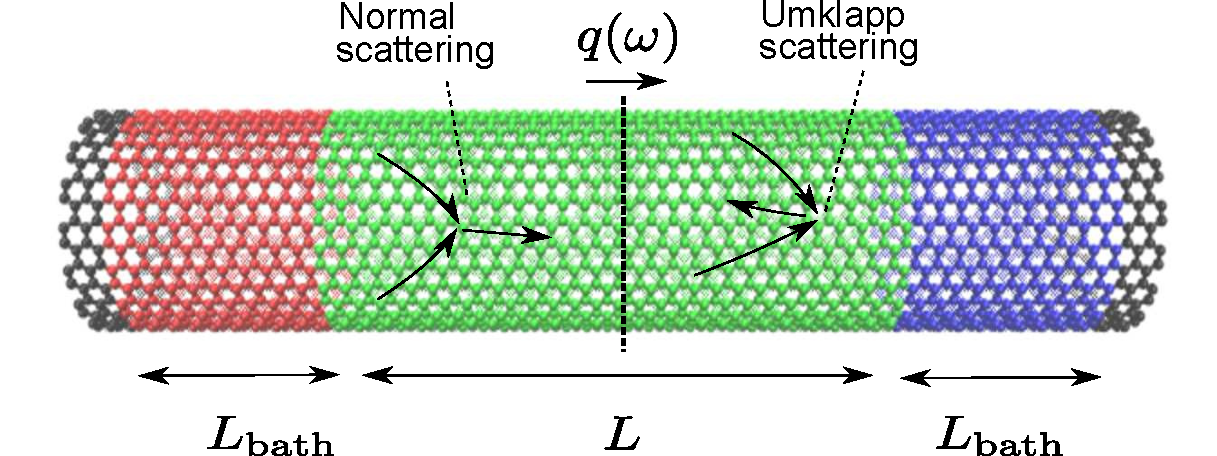
\includegraphics[width=.89\columnwidth]{pics/cnt_fig1-crop.pdf} 
  \caption{Schematic illustration of the NEMD setup used for determining the length-dependent thermal conductivity and phonon mean free paths in carbon nanotubes. When traversing the tube, phonons undergo both normal and Umklapp processes giving rise to length-dependent spectral heat current $q(\omega)$ in the tube. From the $L$-dependence of $q(\omega)$, one can determine the mean free paths at each frequency as described in \citepub{cnt}. Figure reprinted with publisher's permission from \citepub{cnt}.}  
\label{fig:cnt_fig1}
 \end{center}
\end{figure}

Carbon nanotubes have a very high thermal conductivity in the range 500-5000 W/mK \cite{marconnet13}, and their thermal conductivity has been found to increase as a function of tube length in tubes as long as 5 $\upmu$m \cite{chang08} and, very recently, even in tubes as long as 1 mm \cite{chang_personal}. Theoretical understanding of the limits of ballistic heat transfer in carbon nanotubes is of crucial importance for their applications in, e.g., thermal management \cite{biercuk02,huang05}. The goal of \citepub{cnt} was to shed insight to the ballistic limits of thermal conductivity in pristine nanotubes by determining the spectral contributions to the thermal current \eqref{eq:th_spectral_curr} in tubes of different lengths $L$ from atomistic simulations. \change{From the length-dependent current $q(\omega;L)$, we first determined the generalized phonon transmission function}
\begin{equation}
 \ca{T}(\omega) = \frac{q(\omega;L)}{k_B \Delta T}, \label{eq:Tomega_L}
\end{equation}
\change{which is essentially the phonon transmission probability through a tube of length $L$ summed over all propagating modes at angular frequency $\omega$. We then determined the mean free paths $\Lambda(\omega)$ by fitting the length-dependent transmission \eqref{eq:Tomega_L} to the equation }\cite{datta,wang06_apl,savic08_prl}
\begin{equation}
 \ca{T}(\omega) = \frac{M(\omega)}{1+L/\Lambda(\omega)}.
\end{equation}
\change{Here $M(\omega)$ is the number of propagating modes in the nanotube in the ballistic limit.}

 %This length-dependence was used to calculate frequency-dependent phonon mean free paths. % The simulated tube lengths exceed 

Figure \ref{fig:cnt_fig1} shows the schematic illustration of the NEMD setup used for carbon nanotubes of (10,10) chirality. Regions of length $L_{\textrm{bath}}=10$ nm were coupled to Langevin thermostats at temperatures $T+\Delta T/2$ and $T-\Delta T/2$ to drive heat current through the tube, and the frequency-dependent phonon mean free paths were determined from the decrease of the non-equilibrium spectral heat current \eqref{eq:th_spectral_curr} at different frequencies as a function of tube length $L$. The decrease in spectral current arises from anharmonic interactions, which are fully accounted for by the non-linear terms of the optimized Tersoff potential used for modeling carbon-carbon interactions \cite{tersoff88a,lindsay10}. In contrast to equilibrium mean free paths, which characterize the equilibrium scattering lengths arising from the combined effect of normal and Umklapp processes \cite{mcgaughey04}, the mean free paths determined from NEMD \textit{directly reflect the resistance to the heat flow} (expected to be dominated by Umklapp processes). % For a detailed account of the method, we refer to \citepub{cnt}.


\begin{figure}[tb]
 \begin{center}
  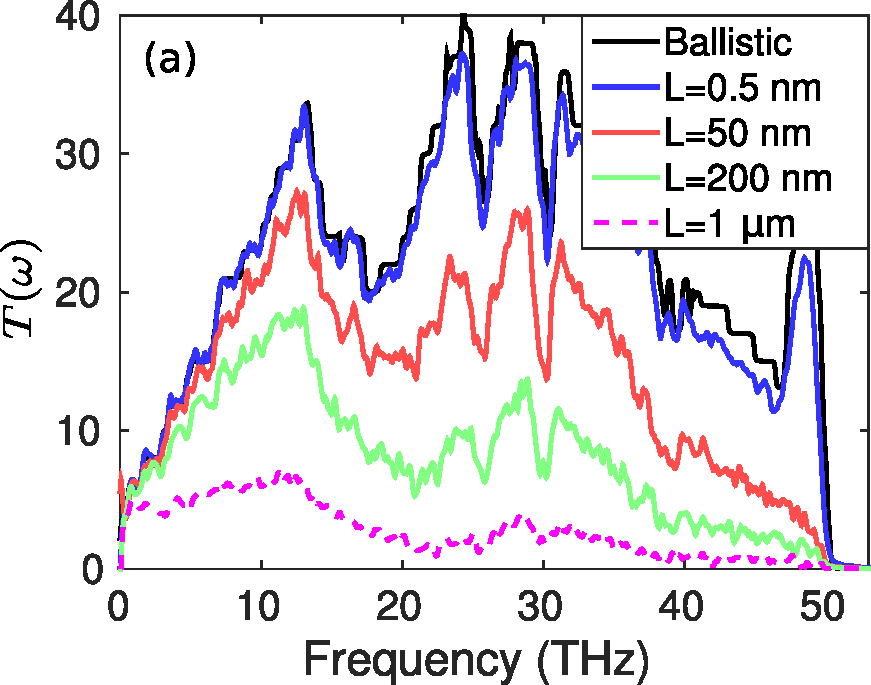
\includegraphics[width=.49\columnwidth]{pics/cnt_fig2_mod.pdf} 
  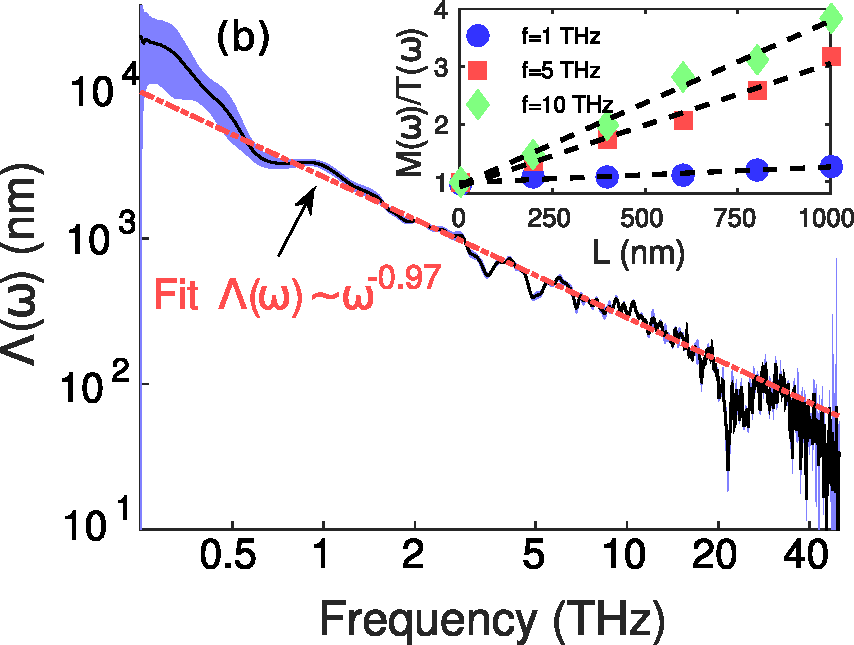
\includegraphics[width=.49\columnwidth]{pics/cnt_fig4_new.pdf} 
  \caption{(a) Generalized phonon transmission function $\ca{T}(\omega)=q(\omega)/(k_B\Delta T)$ for different tube lengths at $T=300$ K. Increasing the tube length reduces the transmission due to anharmonic scattering. For $L=0.5$ nm, phonon transmission is nearly equal to the ballistic value determined by counting the number of propagating modes in the nanotube. (b) Log-log plot of the mean free path $\Lambda(\omega)$ at $T=300$ K, determined from the slope of the inverse transmission function as a function of tube length $L$ as illustrated by the dashed lines in the inset. The shaded regions in the main figure correspond to the 92.5\% confidence interval for the slope. Below 0.25 THz, the confidence interval is large due to numerical uncertainties, preventing the determination of mean free paths at the lowest frequencies. Figure reprinted with publisher's permission from \citepub{cnt}.}  
\label{fig:cnt_fig2}
 \end{center}
\end{figure}

Figure \ref{fig:cnt_fig2}(a) shows the generalized phonon transmission function $\ca{T}(\omega)$ for different tube lengths $L$. For $L=0.5$ nm, the transmission probability of each mode is unity and the generalized phonon transmission is nearly equal to the number of propagating phonon modes (black solid line). As the tube length increases, anharmonic scattering reduces the transmission. This reduction is strongest at high frequencies, suggesting that the mean free path decreases as a function of frequency, which is reasonable considering the larger phase-space available for phonon-phonon scattering at high frequencies \cite{ziman}.

Phonon mean free paths are plotted as a function of frequency in Fig. \ref{fig:cnt_fig2}. The mean free paths are calculated using the fitting procedure depicted in the inset of Fig. \ref{fig:cnt_fig2} and described in detail in \citepub{cnt}. The results show that the mean free paths obey a power-law $\Lambda(\omega)\propto \omega^{-\alpha}$ as a function of frequency in a large frequency interval, with a different exponent $\alpha\approx 0.97$ than the value $\alpha=2$ used earlier \cite{wang06_apl} to phenomenologically describe the ballistic-diffusive transition in carbon nanotubes. \change{This disagreement is not surprising, because the value $\alpha=2$ has been derived \cite{ziman} for three-dimensional bulk systems and is therefore expected to break down in quasi-one-dimensional nanotubes. The exact value of the exponent $\alpha$ is also sensitive to the detailed geometry of the system, as suggested by recent results for one-dimensional anharmonic chains, for which the value $\alpha\approx 1.67$ has been found \cite{saaskilahti15b}}. At low frequencies, the mean free paths shown in Fig. \ref{fig:cnt_fig2} exceed 10 $\upmu$m, in agreement with the strong length-dependence of the experimentally measured thermal conductivity in nanotubes as long as $5$ $\upmu$m \cite{chang08}. 

The numerical results for the phonon mean free paths show that thermal conduction in carbon nanotubes is partially ballistic at least up to micrometer scale. At very low frequencies ($f\lesssim 0.1$ THz), the mean free paths might extend even up to millimeter scale. This conclusion contradicts earlier simulation results \cite{thomas10b} showing the convergence of thermal conductivity in 1 $\upmu$m long nanotubes. The disagreement most likely originates from the different interatomic potential used in the simulations: the REBO potential \cite{brenner02} employed in Ref. \cite{thomas10b} is known to underestimate the thermal conductivity of carbon nanomaterials \cite{salaway14}. 

% Analysis of the spectral thermal conductivity $\kappa(\omega)=Lq(\omega)/\Delta T$ in \citepub{cnt} reveals that modes with frequencies 

% \textbf{DISCUSS THE LIMITS OF BALLISTIC CONDUCTION}

\subsection{Thermal conductivity reduction in twinning nanowires}

\label{sec:results_twinning}

Efficient thermoelectric conversion generally requires materials with low thermal conductivity and high electronic conductivity \cite{majumdar04}. Nanostructuring is known to be an effective way to reduce the thermal conductivity by increasing phonon scattering \cite{vineis10,shakouri11}. In silicon nanowires, for example, phonon scattering from the rough nanowire surfaces and the reduction in the phonon group velocity due to spatial confinement \cite{balandin98} reduce the thermal conductivity by two orders of magnitude compared to the bulk value \cite{hochbaum08,boukai08}, thereby increasing the thermoelectric figure of merit \cite{chen} close to unity. To investigate possibilities to increase the thermoelectric efficiency of Si nanowires even further, \citepub{twinning} studied the effect of periodic twinning stacking faults \cite{algra08,caroff09} on the thermal properties of Si nanowires.


\begin{figure}[tb]
 \begin{center}
  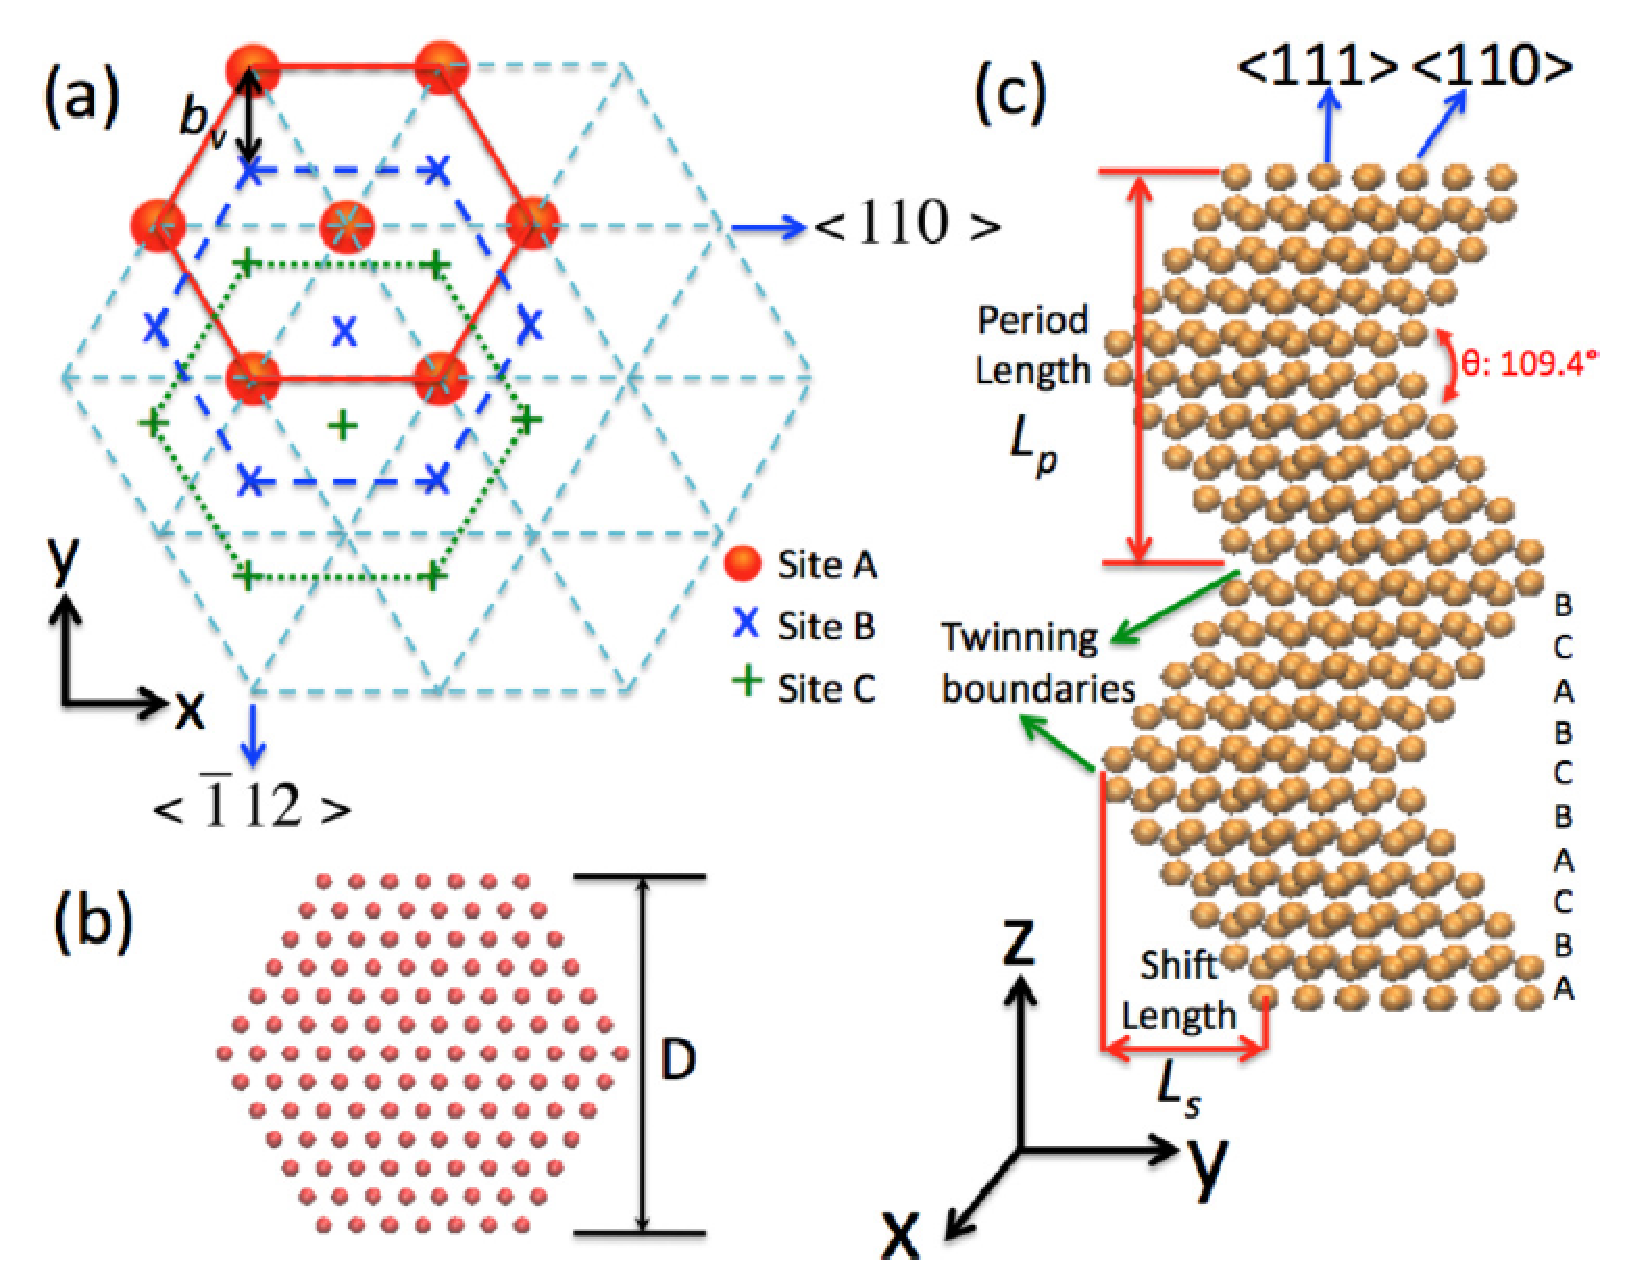
\includegraphics[width=.89\columnwidth]{pics/twinning_fig1.pdf} 
  \caption{(a) Schematic illustration of stacking in the close-packed silicon lattice. Stacking fault occurs when the stacking sequence ABCABC is locally changed to ABCBAC. (b) Cross-section of the nanowire. (c) Silicon nanowire with twinning boundaries. The period length is denoted by $L_p$ and the ''shift length'' $L_s$ is related to $L_p$ by $L_s=(L_p/2)\cot(\theta/2)$, where $\theta=109.4^{\circ}$. The figure also illustrates the perturbation of the ABCABC... stacking sequence at the twinning boundaries. Figure reprinted with publisher's permission from \citepub{twinning}.}  
\label{fig:twinning_fig1}
 \end{center}
\end{figure}

Twinning stacking faults \cite{cahn54} are common defects appearing in the vapor-liquid-solid growth of nanowires made of group IV and group III-V nanowires \cite{johansson06,xiong06,davidson07,algra08}. At a twinning interface, the crystallographic orientation of the nanowire changes without leaving any dangling bonds \cite{korgel06}. In the Si nanowire illustrated in Fig. \ref{fig:twinning_fig1}, the twinning interface essentially joins two nanowires with different stacking orders as depicted in Figs. \ref{fig:twinning_fig1}(a) and (c), giving rise to periodically repeating kinks in the nanowire. Such periodic kinks perturb phonon propagation in the nanowire and are expected to therefore reduce the thermal conductivity. Periodically twinned Si nanowires have been recently grown experimentally \cite{ruffino15}.

The computational NEMD setup of \citepub{twinning} was similar as for the carbon nanotubes considered in \citepub{cnt}, with the exception that Langevin heat baths were replaced by deterministic Nos\'e-Hoover thermostats \cite{nose84,hoover85} and interatomic potential was replaced by the Stillinger-Weber potential \cite{stillinger85} modeling silicon-silicon interactions. The cross-section of the nanowires was chosen to be hexagonal with diameter $D$ as shown in Fig. \ref{fig:twinning_fig1}(b). The twinning period is denoted by $L_p$, corresponding to the ''shift length'' $L_s=(L_p/2)\cot(\theta/2)$, where $\theta=109.4^{\circ}$ is the kink angle as shown in Fig. \ref{fig:twinning_fig1}(c). 


\begin{figure}[tb]
 \begin{center}
   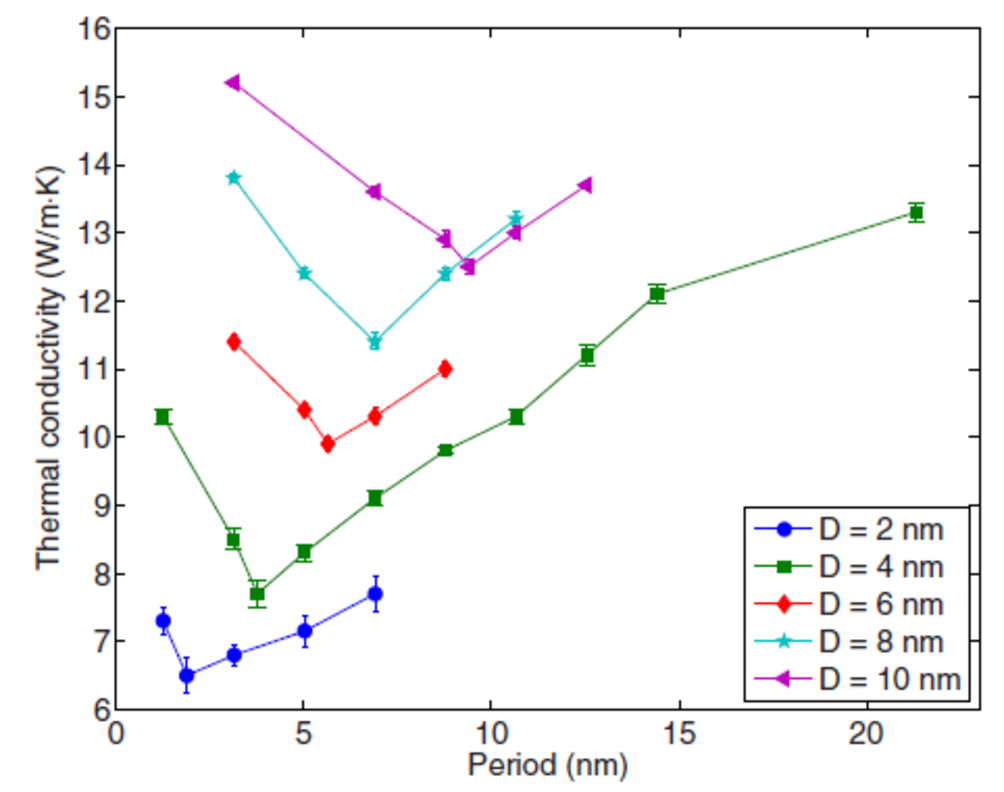
\includegraphics[width=.89\columnwidth]{pics/twinning_fig2a_mod.pdf} 
  \caption{Thermal conductivity of silicon twinning nanowires at $T=300$ K as a function of period length $L_p$ for different diameters $D$. For each diameter $D$, there is a corresponding minimum in the thermal conductivity as a function of period length. The minimum arises from the competition between geometric and anharmonic effects as shown in \citepub{twinning}. Figure reprinted with publisher's permission from \citepub{twinning}.}  
\label{fig:twinning_fig2}
 \end{center}
\end{figure}

Thermal conductivity of the twinning nanowires as a function of period $L_p$ are shown in Fig. \ref{fig:twinning_fig2} for different diameters $D$. For each diameter, there is a corresponding period length with a minimum in the thermal conductivity. Lowest conductivity was found for the period length $L_p\approx 0.95D$, corresponding to the shift length $L_s=D/3$. The detailed mechanisms behind the minimum thermal conductivity were analyzed in detail in \citepub{twinning}, with the conclusion that it \change{essentially} arises from the \change{interplay of} geometric and anharmonic scattering. \change{When the period is very small, the twinning as (small) surface roughness and resistance to heat flow is dominated by anharmonic effects. When the period gets longer, phonons are forced to change propagation direction at the kinks, increasing the geometric scattering and reducing the conductivity. When the period is very long, however, scattering at kinks becomes infrequent and the resistance is again determined by anharmonic scattering. Therefore, a minimum in the conductivity as a function of period is expected.}

The results of \citepub{twinning} show that periodical twinning can reduce the thermal conductivity of Si nanowires by 65\% compared to the straight wire.  Because the reduction of electronic conductivity is expected to be smaller due to the smaller wavelength of electrons, twinning could be used to enhance the thermoelectric performance of Si nanowires. To reduce thermal conductivity even further, periodically twinned Si nanowires could be partially amorphized \cite{donadio09} or coated with germanium \cite{hu11}. 

\section{Interference effects in phononic thermal conduction across point contacts}
\label{sec:results_interference}

For applications in thermionic \cite{zeng06}\cite{westover08} and thermophotonic \cite{oksanen08} cooling as well as thermophotovoltaic generation \cite{dimatteo01}, good thermal insulation between two bulk materials separated by a nanoscale gap is required. While a pure vacuum gap would be optimal in preventing the propagation of phonons through the gap, practical applications require structural support in the form of nanoscale point contacts bridging the gap. Such point contacts conduct heat and can therefore disturb thermal insulation. Thermal conduction properties of point contacts between bulk materials have therefore become of both theoretical \cite{saha07} and experimental \cite{bartsch12} interest in recent years.

Because the feature sizes of nanoscale point contacts can be comparable to thermal phonon wavelengths \change{and coherence lengths}, interference effects can play an important role in thermal conduction across the contact. Identification of interference effects in point contacts could possibly be exploited for thermal conductivity engineering in the same way as, e.g., in phononic crystals \cite{maldovan13}.

\begin{figure}
\begin{center}
 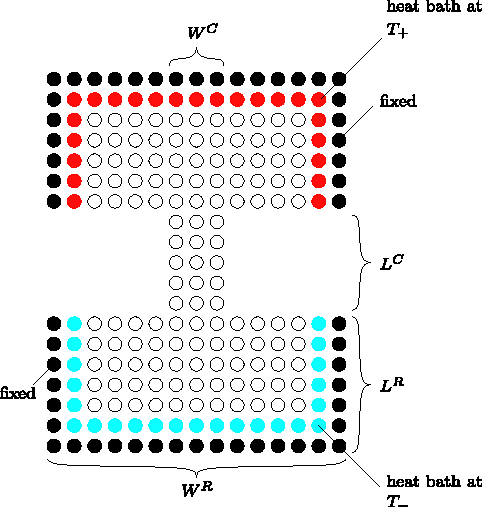
\includegraphics[width=.60\columnwidth]{pics/fpu_fig1_mod.pdf}
 \caption{Schematic illustration of the simulation setup for a point contact in a two-dimensional square lattice. Figure reprinted with publisher's permission from \citepub{fpu}.}
\label{fig:fpu_fig1}
\end{center}
\end{figure}

To investigate thermal conduction and interference effects in point contacts, we performed NEMD simulations using the simulation setup schematically illustrated in Fig. \ref{fig:fpu_fig1}. Atoms were placed in a square lattice, with the particles at the boundaries of the bulk parts at the top or bottom being either fixed (black circles) or coupled to Langevin baths at temperature $T_+$ (red circles) or $T_-$ (cyan circles). In \citepub{fpu}, the large bulk parts were connected by a rectangular point contact that is $L^C$ atoms long and $W^C$ atoms wide. Triangular and discoidal shaped point contacts were considered in \citepub{fpu2}. 

Lattice dynamics in the setup of Fig. \ref{fig:fpu_fig1} was modeled by coupling all nearest-neighbor atom pairs by anharmonic springs (not shown), whose potential energies include both quadratic and quartic terms. This potential was used by Fermi, Pasta and Ulam to investigate thermalization in one-dimensional systems \cite{fermi55} and is therefore called Fermi-Pasta-Ulam potential. The simple form of the Fermi-Pasta-Ulam potential allows for scaling the anharmonicity by a corresponding scaling in temperature, so one can present results for a single value of anharmonicity parameter without loss of generality. This scaling and other simulation details are presented in \citepub{fpu}.


\begin{figure}
\begin{center}
 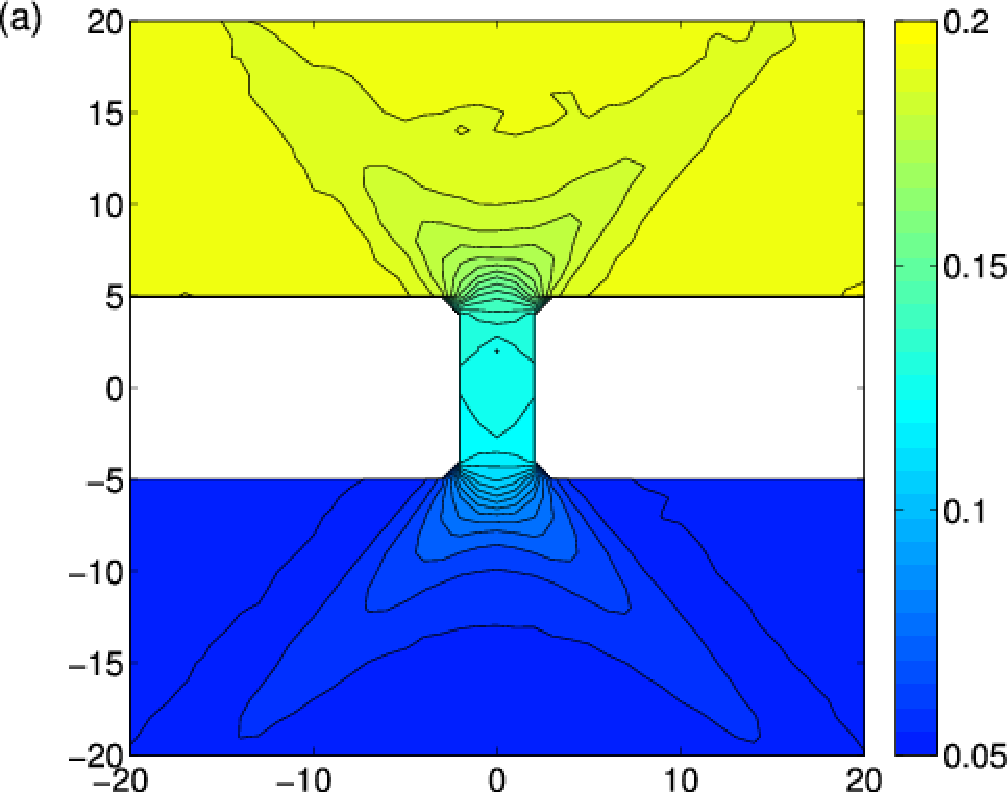
\includegraphics[width=.49\columnwidth]{pics/fpu_fig2a.pdf}
  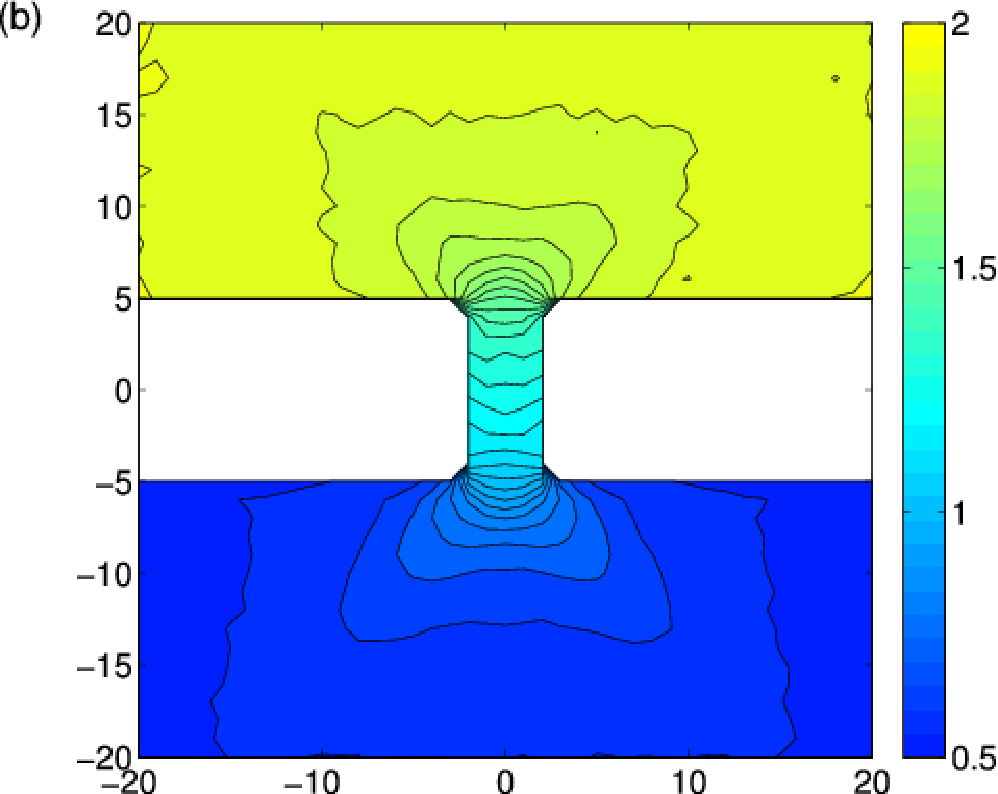
\includegraphics[width=.49\columnwidth]{pics/fpu_fig2b.pdf}
 \caption{Kinetic temperature profile at (a) low temperature ($T_+=0.20$, $T_-=0.05$) and (b) high temperature ($T_+=2.0$, $T_-=0.5$). The bulk size is $W^R=161$, $L^R=80$ and the contact size $W^C=5$, $L^C=9$ (see Fig. \ref{fig:fpu_fig1}). The labels on the horizontal and vertical axes mark the atom indices. Figure reprinted with publisher's permission from \citepub{fpu}.}
\label{fig:fpu_fig2}
\end{center}
\end{figure}

Figure \ref{fig:fpu_fig2} shows the kinetic temperature $T_i^{\textrm{kin}}=\langle mv_i^2 \rangle/k_B$ at each atomic site $i$ in a contour plot at (a) low temperature and (b) high temperature for a rectangular contact of length $L^C=9$ and width $W^C=5$. \change{Temperatures are given in the units of $T_0=m^2\omega_0^4/\beta$, where $\omega_0$ is the resonance frequency of the springs connecting the atoms and $\beta$ is the potential anharmonicity parameter defined in} \citepub{fpu}. At low temperature, lattice waves can propagate without losses and, therefore, temperature is nearly constant in the contact. Most notably, the lossless propagation can be seen to induce wavelike-features in the kinetic temperature profile in the bulk parts, with directional features along the $\langle 11 \rangle$ crystal directions. Such features contradict Fourier's law predicting a highly symmetric temperature profile with no directional features (not shown). When temperature is increased [Fig. \ref{fig:fpu_fig2}(b)], the directional features vanish and temperature profile becomes more similar to Fourier's law's prediction. Temperature profile also develops a non-zero gradient inside the contact due to the smaller thermal conductivity.


\begin{figure}
\begin{center}
 %\includegraphics[width=8.6cm]{../scbaths_paper_re_resubmission/pic1.ps}
 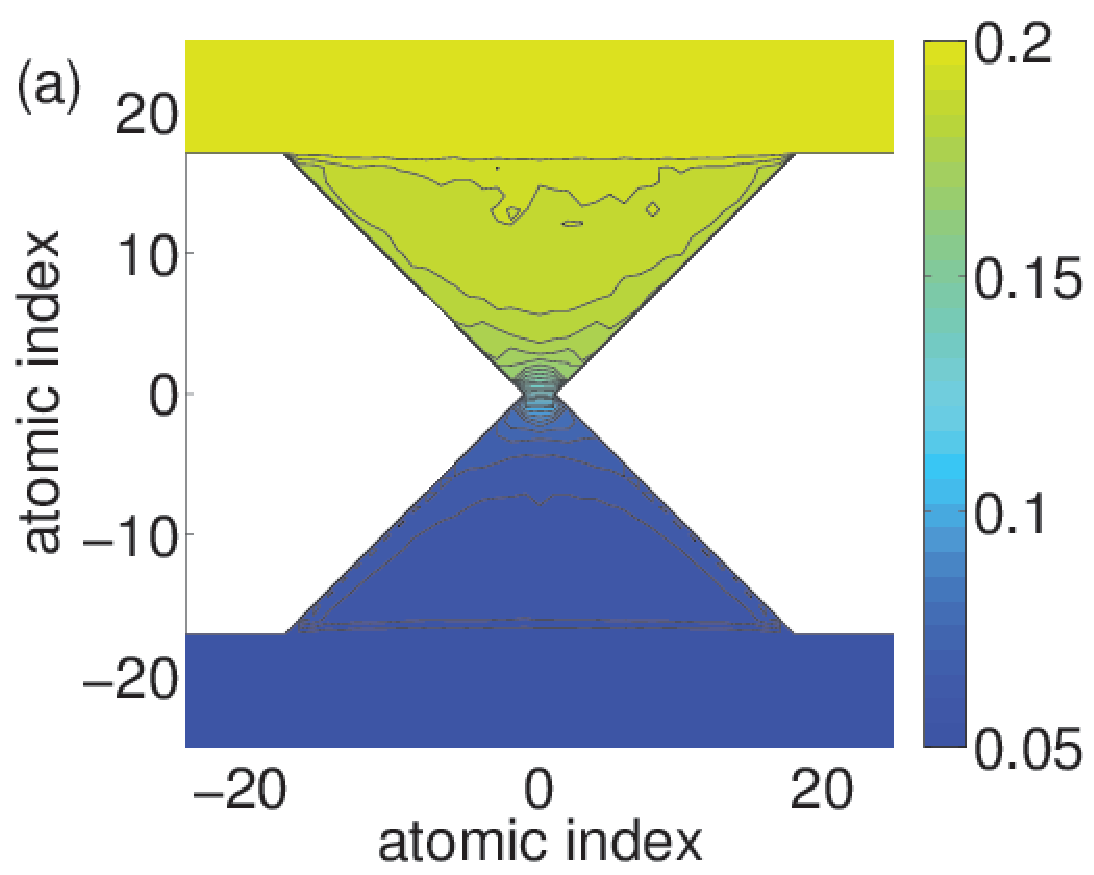
\includegraphics[width=.49\columnwidth]{pics/aip_fig5a.pdf}
 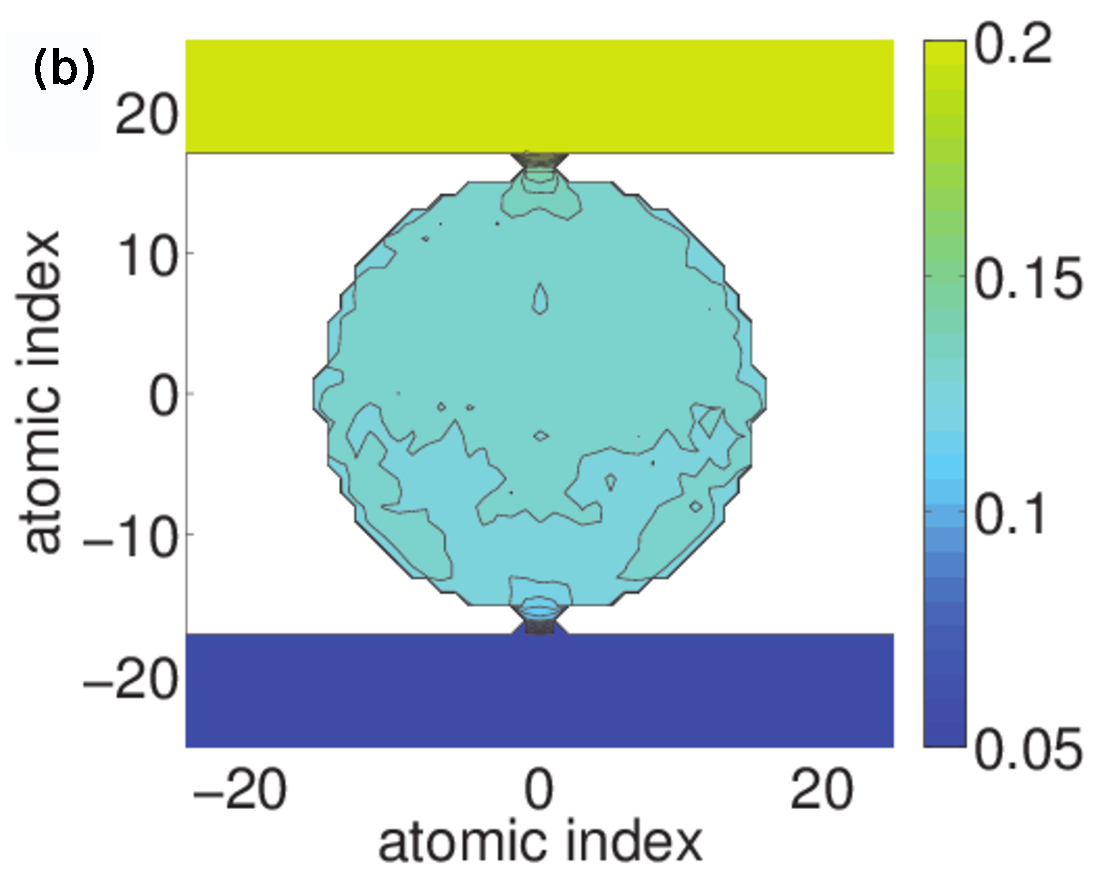
\includegraphics[width=.49\columnwidth]{pics/aip_fig6a_mod.pdf}
 %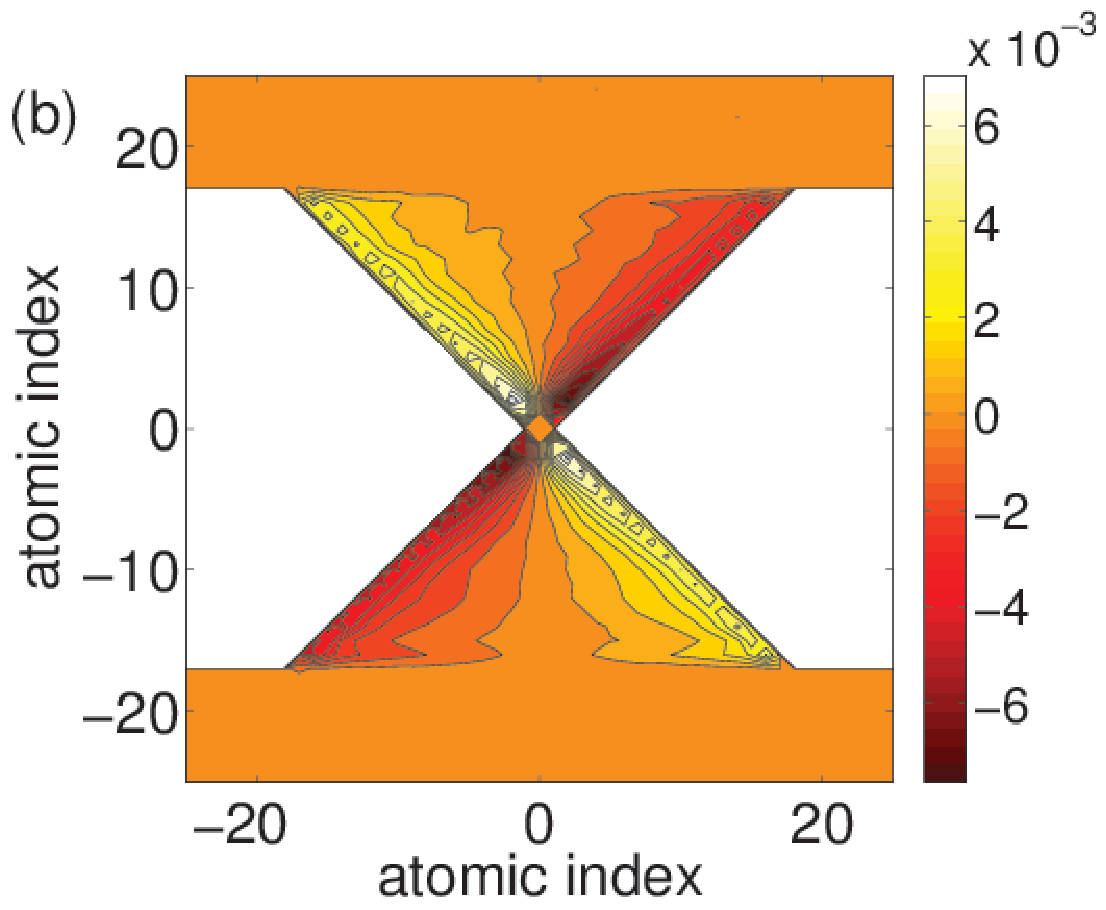
\includegraphics[width=.49\columnwidth]{pics/aip_fig5b.pdf}
 \caption{Kinetic temperature profile in (a) triangular and (b) discoidal contacts at low temperature. Figure reprinted with publisher's permission from \citepub{fpu2}.}
\label{fig:aip_figs56}
\end{center}
\end{figure}

To investigate the effects of the contact geometry on interference effects at low temperatures, calculations were performed also for hour-glass shaped and discoidal contacts. \change{Such variations in the geometry are interesting, because the point contact could be formed, e.g., by nanoparticles deposited in the vacuum gap between the materials.} Kinetic temperature profiles for the hour-glass shaped and discoidal geometries are shown in Fig. \ref{fig:aip_figs56}. For small contact areas in the triangular and discoidal contacts, temperature profiles in the bulk parts are essentially constant due to the small thermal contact between the upper and lower parts of the structure. In the triangular point contact, temperature changes nearly linearly as the contact becomes narrower. Spatial analysis of the local heat current presented in \citepub{fpu2} reveals that heat flows mainly along the edges of the triangles. In the discoidal geometry of Fig. \ref{fig:aip_figs56}(b), which could represent a nanoparticle sandwiched between two materials, temperature profile is again nearly flat inside the center region, with only small spatial variations in temperature. However, local heat currents inside the center region, shown in \citepub{fpu2}, are strongly direction-dependent, with similar enhancement in $\langle 11\rangle$ direction as in the temperature profile of Fig. \ref{fig:fpu_fig2}(a).

The results show that in the ballistic low-temperature limit, local temperature and heat current profiles can exhibit wavelike-features \change{arising from mode interference and (partially) ballistic conduction}. \change{In future, it would be useful to analyze the mean free paths and transmission probabilities of individual modes to quantitatively understand the origin of directional patterns in different geometries}. Accounting for such directional patterns could enable more efficient engineering of thermal conductivity in nanostructures. It is, however, well known that the effect of quantum statistics neglected by classical MD can be significant at low temperatures. To include quantum statistics, we turn to the quantum-mechanical GF method based on the linearized Langevin equations of motion presented in Sec. \ref{sec:th_eom}

%The results show that in the ballistic low-temperature limit, local temperature and heat current profiles can exhibit wavelike-features with interference patterns. Accounting for such directional patterns could enable more efficient engineering of thermal conductivity in nanostructures. It is, however, well known that the effect of quantum statistics neglected by classical MD can be significant at low temperatures. To include quantum statistics, we turn to the quantum-mechanical GF method based on the linearized Langevin equations of motion presented in Sec. \ref{sec:th_eom}.

\section{Langevin modeling of phononic and photonic energy transfer}
\label{sec:results_gf}

As discussed in Sec. \ref{sec:th_eom}, solving the linearized Langevin equations \eqref{eq:th_eom1}, \eqref{eq:th_eom2}, and \eqref{eq:th_eom3} in terms of the GF allows for heat transfer modeling that accounts for wave interference, quantum statistics, and even dissipative losses in terms of a frequency-independent relaxation rate. In this thesis, GF method is applied to investigate (i) quantum thermal transport through point contacts in Subsection \ref{sec:results_schb} and (ii) cavity-en\-hance\-ment of electromagnetic energy transfer rates between SiC nanoparticles in Subsection \ref{sec:results_cavity}. 

\subsection{Quantum effects in point contacts}
\label{sec:results_schb}

Application of the linearized Langevin equation \eqref{eq:th_eom1} for lossy phonon transport is closely related to the self-consistent heat bath model \cite{bolsterli70}, discussed in detail in this Subsection. Whereas earlier works have applied the model to simple one-dimensional systems (see, e.g., Refs. \cite{bolsterli70,visscher75,dhar03,dhar06,segal09,bandyopadhyay11}) with a finite number of atoms, \citepub{gf} extended the model to more complex geometries with an infinite number of atoms.  

The setup of \citepub{gf} is schematically illustrated in Fig. \ref{fig:schb_setup}. The setup consists of a center region with a finite number of atoms and left and right leads with possibly an infinite number of atoms. All atoms are coupled to local Langevin baths mimicking all interaction events driving the system towards local thermal equilibrium \cite{bolsterli70}. In the center region of Fig. \ref{fig:schb_setup}(a), a point contact acts as a scattering center for phonons coming in from the left and right leads. In the vicinity of the contact, bath temperatures are unknown. Following the self-consistent heat bath model \cite{bolsterli70}, these temperatures are determined self-consistently from the requirement that the heat current to each bath vanishes. The requirement of zero heat current to local baths ensures that the heat current flowing in the system is conserved at each atom site, a natural requirement in the steady-state in the absence of coupling to other carriers such as electrons.

Away from the scattering region, the baths are set to prescribed temperatures $T_L$ and $T_R$. Whereas earlier works \cite{dhar06} have modeled lattice dynamics in the leads as completely lossless, which induces an acoustic mismatch between the lossless leads and the lossy center region, the setup of Fig. \ref{fig:schb_setup} eliminates this mismatch by including losses for the leads as well.  

\begin{figure}
\begin{center}
 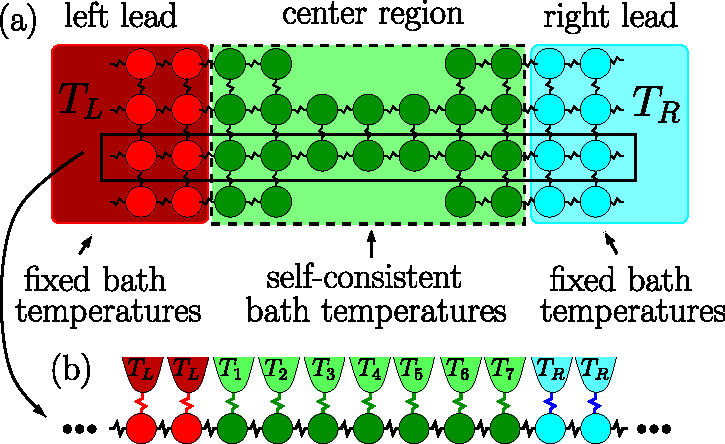
\includegraphics[width=.99\columnwidth]{inkscape/gf_fig1.pdf}
 \caption{A schematic illustration of the self-consistent heat bath model for a constriction in a two-dimensional rectangular lattice. The system consists of the left lead, the center region, and the right lead. All atoms are coupled to Langevin heat baths, shown explicitly for one cross section in (b). Whereas the temperatures of the Langevin baths have prescribed values $T_L$ and $T_R$ in the left and right lead, the bath temperatures are determined self-consistently in the center region from the requirement that the thermal current to each bath is zero \cite{bolsterli70}. Reprinted from \citepub{gf} with publisher's permission.}
\label{fig:schb_setup}
\end{center}
\end{figure} 

The calculation of heat currents starts from the Langevin equation of motion \eqref{eq:th_eom1} for each atom $i$ with interatomic force constants $\bb{K}_{ij}$ determined by the interatomic potential energy function. The relaxation rate $\gamma$ is chosen to correspond to known phonon life-times. It is shown in \citepub{gf} that solving the equations of motion for the leads and substituting to the equations for the center region allows for replacing the leads by \textit{single} Langevin heat baths at temperatures $T_L$ and $T_R$, which reduces the number of degrees of freedom to those in the center region. The microscopic details of acoustically matched lattice dynamics in the leads are fully captured by the lead self-energy functions $\Sigma^L(\omega)$ and $\Sigma^R(\omega)$. Microscopic definitions of the self-energy function in terms of the lead GF and the fluctuation-dissipation theorem for the corresponding Langevin noises are presented in detail in \citepub{gf}.

By following the procedure presented in Sec. \ref{sec:th_bathcurrents}, one can calculate the heat currents flowing to baths in terms of the center region's GF $\bb{G}(\omega)$. By setting the heat current equal to zero for the local baths in the center region, one gets a non-linear system of equations for the bath temperatures. This system of equations can be solved by, e.g., using Newton-Raphson method \cite{bandyopadhyay11} or resorting to linearizing approximations \cite{segal09}. It is shown in \citepub{gf} that the requirement of vanishing heat current to the baths is equivalent to an intuitive thermal balance condition between kinetic and potential energies. Similar thermal balance condition was recently reported for local photon number in fluctuational electrodynamics \cite{partanen14}. 

\begin{figure}
 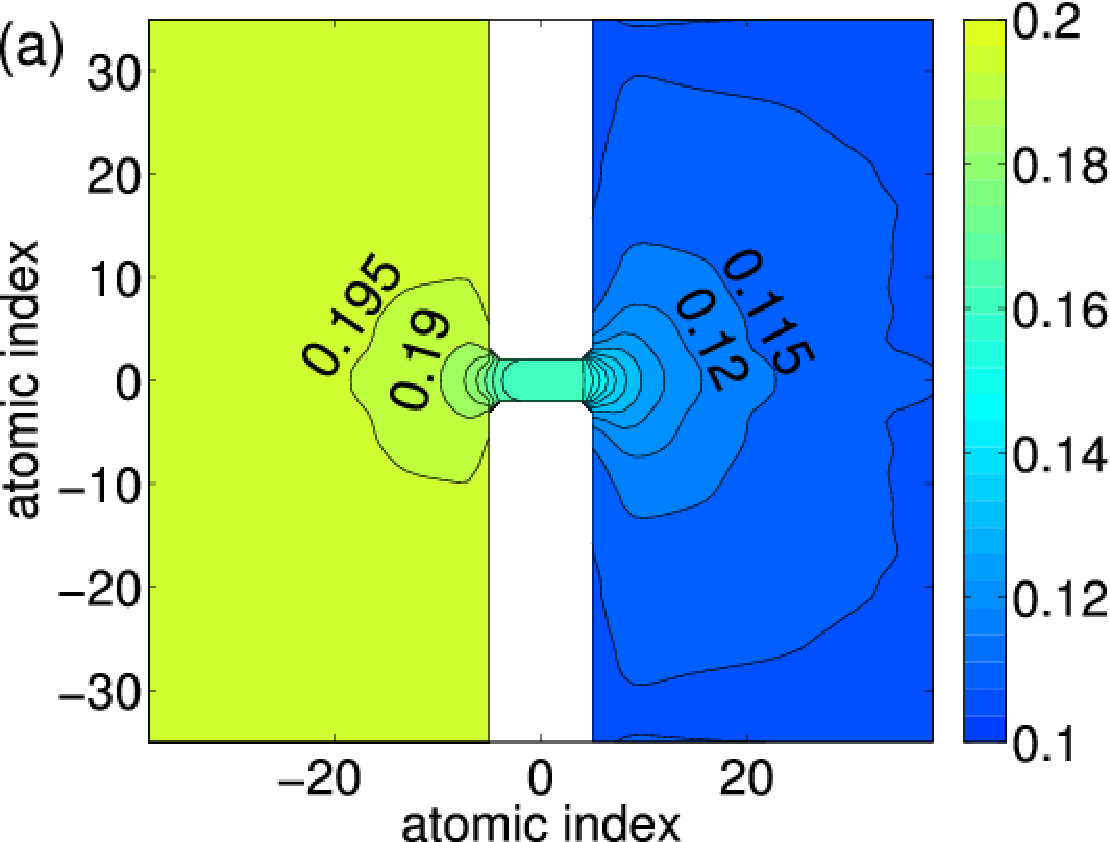
\includegraphics[width=.49\columnwidth]{pics/gf_fig7a.pdf}
 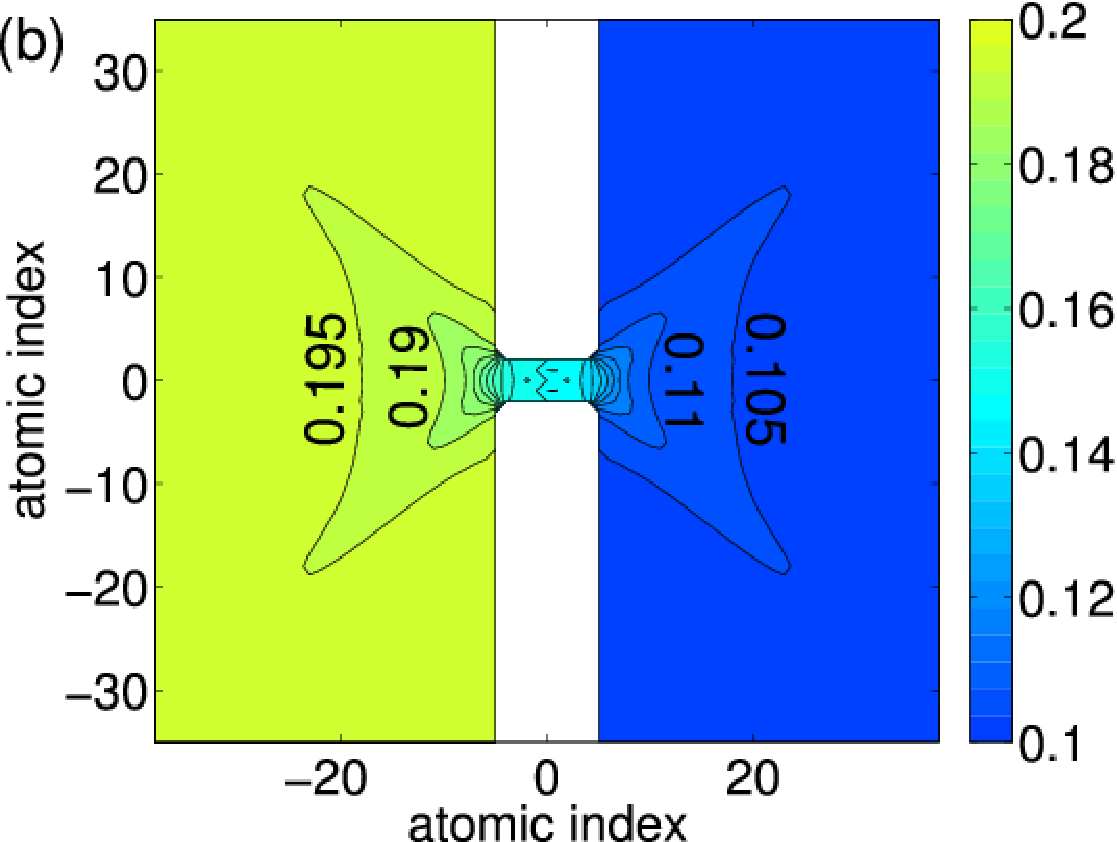
\includegraphics[width=.49\columnwidth]{pics/gf_fig7b.pdf}
 \caption{Self-consistent local bath temperature profiles in a rectangular contact connecting two square lattices. Lead temperatures are $T_L=0.2$ and $T_R=0.1$. Figures show temperature profiles for (a) quantum and (b) classical statistics. Friction parameter is $\gamma=0.01$, corresponding to nearly ballistic transport. Figure reprinted with publisher's permission from \citepub{gf}.}
 \label{fig:gf_fig7}
\end{figure}

As an application of the formalism, we investigated quantum effects in thermal transport through a rectangular point contact in a square lattice, considered in Sec. \ref{sec:results_interference} by classical MD. Nearest neighbors were connected by harmonic springs and weak dissipative losses were included through the bath dissipation parameter $\gamma=0.01$ in the units of spring resonance frequency (see \citepub{gf}). Figure \ref{fig:gf_fig7} shows temperature profiles for (a) quantum and (b) classical statistics \change{with lead temperatures $T_L=0.2$ and $T_R=0.1$.} \change{This temperature range should be compared to the Debye temperature of $T_D=2.0$ (defined in Sec. \ref{sec:methods_md}), which exceeds lead temperatures by an order of magnitude. Therefore, the system considered in Fig. \ref{fig:gf_fig7}(a) is deep in the quantum regime.} In this case, the directional features observed in the classical case of Fig. \ref{fig:gf_fig7}(b) and MD results of Fig. \ref{fig:fpu_fig2}(a) can be seen to be washed away by quantum statistics. This suggests that the directional features observed in the classical case arise from high-frequency modes, whose population is overestimated by classical statistics.

To see if interference effects could be observed in a more realistic system, we studied quantum thermal transport through a graphene point contact depicted in Fig. \ref{fig:gf_fig8}(a). Determining temperature profiles for such a system from classical methods such as MD simulation might be very inaccurate due to the high energies of optical phonons in graphene, requiring quantum-mechanical treatment. The drawback of the GF method is that anharmonic phonon scattering is captured only in the mode-independent relaxation time $\gamma^{-1}=1$ ps, which we take to correspond to the experimentally measured phonon life-time \cite{bonini12}. The interatomic force constants $\bb{K}_{ij}$ are taken from the fourth-nearest-neighbor force constant model \cite{saito} with the parameters of Ref. \cite{wirtz04}. 

\begin{figure}
 \begin{center}
 \includegraphics[width=.50\columnwidth]{inkscape/graphene.pdf}
 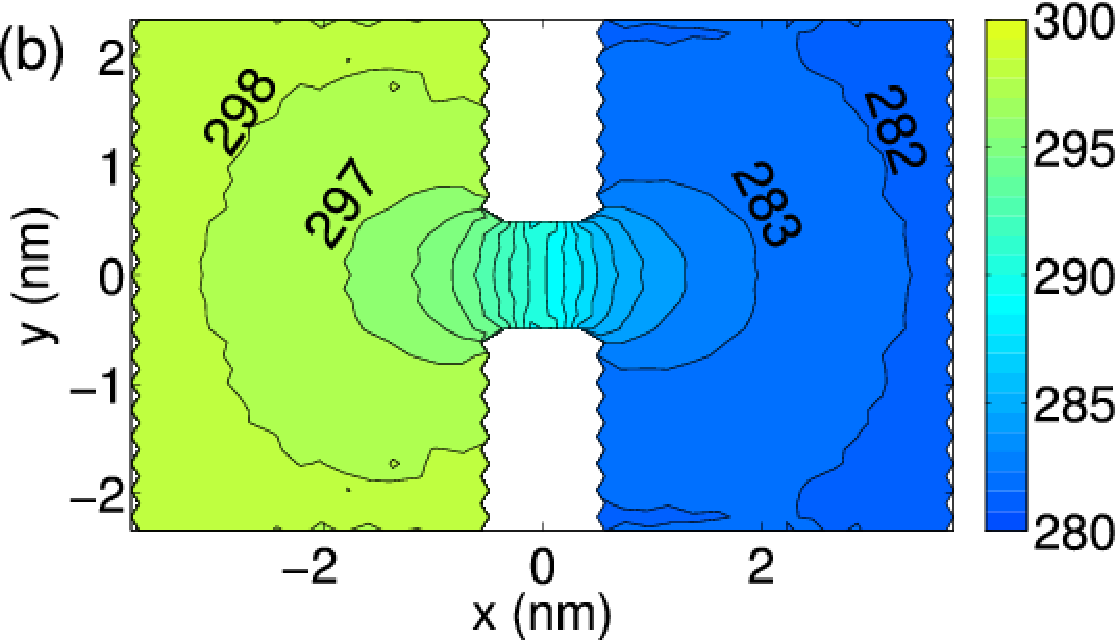
\includegraphics[width=.49\columnwidth]{pics/gf_fig8b.pdf}
 \end{center}
 \caption{(a) Illustration of a point contact in graphene. The leads (red and blue atoms) extend infinitely to the left and right, but the temperatures are determined self-consistently only for the center region (green atoms). (b) Self-consistent bath temperature profiles (K). The semi-infinite leads are at temperatures $T_L=300$ K and $T_R=280$ K. Phonon relaxation time $\tau=1/\gamma$ is set to $1$ ps. Figure (b) reprinted with publisher's permission from \citepub{gf}.}
 \label{fig:gf_fig8}
\end{figure}

The calculated temperature profile in the graphene point contact is plotted in Fig. \ref{fig:gf_fig8}(b) for lead temperatures $T_L=300$ K and $T_R=280$ K. In the considered geometry, there are no visible interference effects in temperature profiles. Quantum effects are observable in the slight asymmetry in temperature profiles at different sides of the junction: purely classical statistics would produce a fully symmetric temperature profile due to the linearity of the self-consistent equations for bath temperatures, as discussed in \citepub{gf}.

The same principles as outlined here for phonon transport can be directly applied to electron transport as well, when the equations of motion for lattice vibrations (Eq. \eqref{eq:th_eom1}) are replaced by the electronic ones (Eq. \eqref{eq:th_eom3}). In electron transport, the self-consistent baths are often referred to as voltage-temperature probes \cite{jacquet09}. Applications of voltage-temperature probe models for describing dissipation effects in electron transport have been so far limited only to one-dimensional geometries \cite{buttiker86,damato90,jacquet09,jacquet12}, although the model can account for wave dynamics, Joule heating as well as thermoelectric effects \cite{roy07} in complicated geometries. Recently, Bergfield \textit{et al.} used the model for investigating quantum temperature oscillations in electrically biased graphene \cite{bergfield15}. 

\subsection{Cavity-modified electromagnetic energy transfer}
\label{sec:results_cavity}

In 1946, Purcell \cite{purcell46} suggested that the emission of electromagnetic radiation from an oscillating dipole could be enhanced by placing the oscillator in a resonant cavity, which effectively increases the electromagnetic density of states and, therefore, the probability of spontaneous emission. The possibility to tune the rate of spontaneous emission was later demonstrated also experimentally \cite{hulet85}\cite{martini87} and is applied, e.g., in resonant cavity light-emitting diodes \cite{schubert92} to enhance the light emission from the active region.

Purcell effect raises the natural question of what are the conditions for similarly tuning the thermal conductance between electromagnetically coupled dielectric bodies. Unlike near-field enhancement of energy transfer, such cavity-tuning is expected to persist at large distances and could be applied, e.g., to (i) enhancing thermal coupling between dielectric bodies, allowing for efficient cooling of hot spots, or (ii) suppressing thermal coupling, preventing undesired propagation of heat.

\begin{figure}
 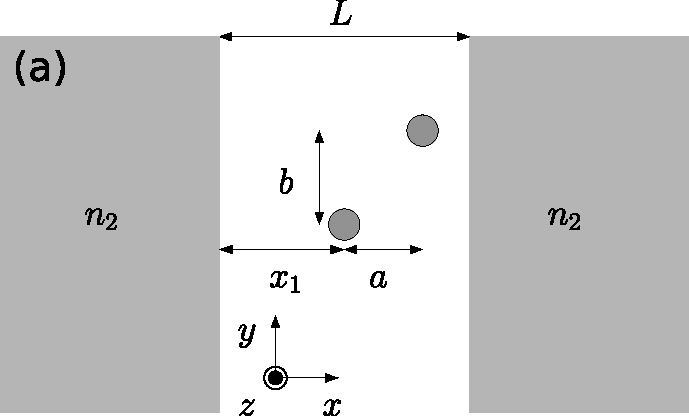
\includegraphics[width=.55\columnwidth]{pics/dipole_fig2.pdf}
 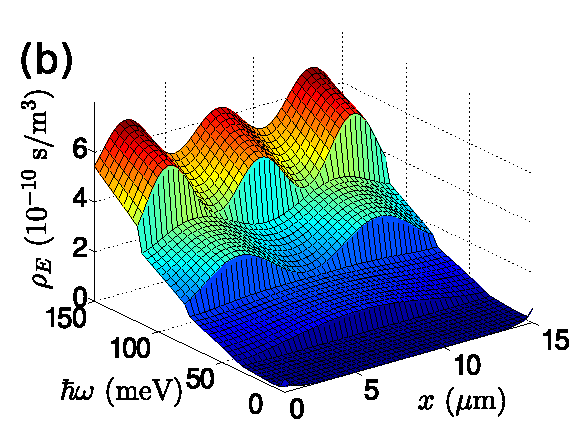
\includegraphics[width=.44\columnwidth]{pics/dipole_fig3a_mod.pdf}
 \caption{(a) Schematic illustration of two nanoparticles located in a mirror cavity of length $L$. One of the particles is located at the middle of the cavity and the position of the second particle is defined by parameters $a$ and $b$ as shown in the figure. The refractive index of the cavity walls is denoted by $n_2$. (b) Electromagnetic density of states as a function of position and energy for a cavity with $L=16$ $\upmu$m and $n_2=2+20i$. The lowest-frequency standing waves have cut-off energies 37.6 meV, 76.3 meV, and 115.1 meV. These modes can couple to the absorption resonance of SiC nanoparticles at $\hbar\omega_r=115.6$ meV. Figure reprinted with publisher's permission from \citepub{dipole}.}
\label{fig:gfm_dipole_system}
\end{figure}

The system studied in \citepub{dipole} is schematically depicted in Fig. \ref{fig:gfm_dipole_system}(a). Two SiC nanoparticles are located in a microcavity formed by two half-spaces with refractive index $n_2=2+20i$ and separated by distance $L$. Due to cavity confinement, the electromagnetic field forms standing waves in the cavity, which can be seen as ''stairs'' in the electromagnetic density of states shown in Fig. \ref{fig:gfm_dipole_system}(b). For $L=16$ $\upmu$m, the lowest-energy standing waves can be excited at 37.6 meV, 76.3 meV, and 115.1 meV. The length of the cavity $L=16$ $\upmu$m is chosen such that only these three low-energy modes can couple electromagnetically to the SiC nanoparticle resonances at 115.6 meV (see below). 

The radius of the nanoparticles is assumed to be $R=250$ nm and the relative dielectric constant $\varepsilon(\omega)$ of SiC is modeled by the Lorentz model \cite{mulet01,spitzer59}. The Clausius-Mossotti polarizabilities of the particles are given by
\begin{equation}
 \alpha^{\textrm{CM}}(\omega)= 4 \pi R^3 \frac{\varepsilon(\omega)-1}{\varepsilon(\omega)+2} \unitdyadic.
\end{equation}
The particles have strong absorption peaks at the phonon-polariton resonance energy $\hbar \omega_r=115.6$ meV corresponding to $\textrm{Re}[\varepsilon(\omega)]=-2$, which forces the interparticle energy transfer to be nearly monochromatic. As discussed above, only three lowest-energy standing waves can be excited in the $L=16$ $\upmu$m cavity at this frequency, and the coupling of the particles to the electromagnetic field therefore depends strongly on the positions of the particles.  

\begin{figure}
 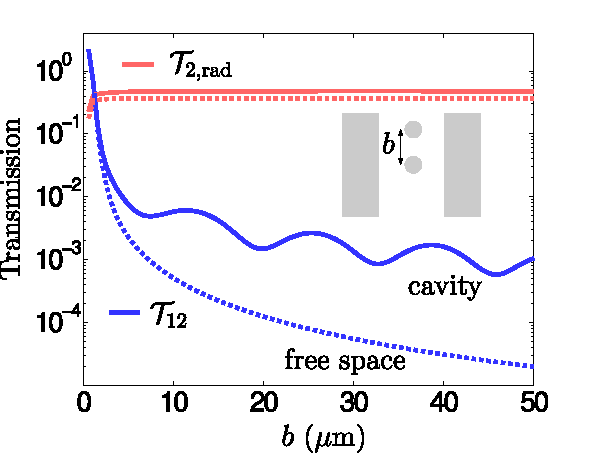
\includegraphics[width=.79\columnwidth]{pics/dipole_fig5.pdf}
 \caption{Energy transmission function $\ca{T}_{12}(\omega_r)$ between two SiC nanoparticles at the nanoparticle resonance frequency $\omega_r$ as a function of vertical separation $b$ (see the inset). The mirror cavity enhances the interparticle thermal conductance and gives rise to interference effects seen as conductance oscillations as a function of distance. The cavity also enhances the coupling between the environment and each dipole, as indicated by the larger dipole-environment transmission function $\ca{T}_{2,\textrm{rad}}(\omega_r)$ with mirror cavity (solid red line) than in free-space (dashed red line). Figure reprinted with publisher's permission from \citepub{dipole}.}
\label{fig:dipole_fig5}
\end{figure}

Figure \ref{fig:dipole_fig5} shows the dipole-dipole transmission $\ca{T}_{12}(\omega_r)$ and the dipole-environment transmission $\ca{T}_{2,\textrm{rad}}(\omega_r)$ at the resonance energy $\hbar\omega_r=115.6$ meV as a function of the vertical distance $b$. The interparticle transmission $\ca{T}_{12}(\omega_r)$ in the cavity (solid blue line) can be seen to exceed the free-space value (dashed blue line) at distances larger than $b\approx 2$ $\upmu$m. In addition, the transmission oscillates as a function of distance due to the interference between electromagnetic cavity modes. As shown in \citepub{dipole}, interparticle thermal conductance can be similarly enhanced also by placing the particles close to a SiC surface supporting surface phonon polaritons.

These results suggest that electromagnetic energy transfer rates between particles can be tuned by modifying the electromagnetic environment, in analogy with the Purcell tuning of radiative emission. Increasing the coupling to the electromagnetic field increases, however, also the thermal coupling to the environment, which may overshadow the interparticle energy transfer. Heat flow from the environment to the particles could be reduced by, e.g., cooling the cavity walls. 

